%Implementation issues have been briefly discussed in \cite{cui_2016_scalcom}. 
This section presents the details of our full-feature implementation of rsMPI, which is an MPI library for Rejuvenating Shadows. 
Similar to rMPI and RedMPI~\cite{ferreira_sc_2011,fiala_2012_sdc}, rsMPI is implemented as a separate layer between MPI and user application. It uses the standard MPI profiling interface to intercept every MPI call and enforces Rejuvenating Shadows logic. In this way, we not only can take advantage of existing MPI performance optimization that numerous researches have spent years on, but also achieve portability across all MPI implementations that conform to the MPI specification.
When used, rsMPI transparently spawns the shadow processes during the initialization phase, manages the coordination between main and shadow processes, and guarantees order and consistency for messages and non-deterministic MPI events.
%Once completed, users should be able to link to the library without any change to existing codes. 

\subsection{MPI rank}
A rsMPI world has 3 types of identities: main process, shadow process, and coordinator process that coordinates between main and shadow. A static mapping between srMPI rank and application-visible MPI rank is maintained so that each process can retrieve its identity. For example, if the user specifies $N$ processes to run, rsMPI will translate it into $2N + K$ processes, %where $K$ is the number of shadowed sets. Then the first $N$ ranks will be the mains, the next $N$ ranks be the shadows, and the last $K$ ranks be the coordinators. 
with the first $N$ ranks being the mains, the next $N$ ranks being the shadows, and the last $K$ ranks being the coordinators. 
We also statically group the processes into shadowed sets according to a user configuration file. Figure~\ref{fig:logical_org} shows an example rsMPI world with 16 application-visible processes grouped into 4 shadowed sets. Using the MPI profiling interface, we added wrapper for MPI\_Comm\_rank() and MPI\_Comm\_size(), so that each process (main or shadow) gets its correct execution path.

\begin{figure}[!t]
  \begin{center}
      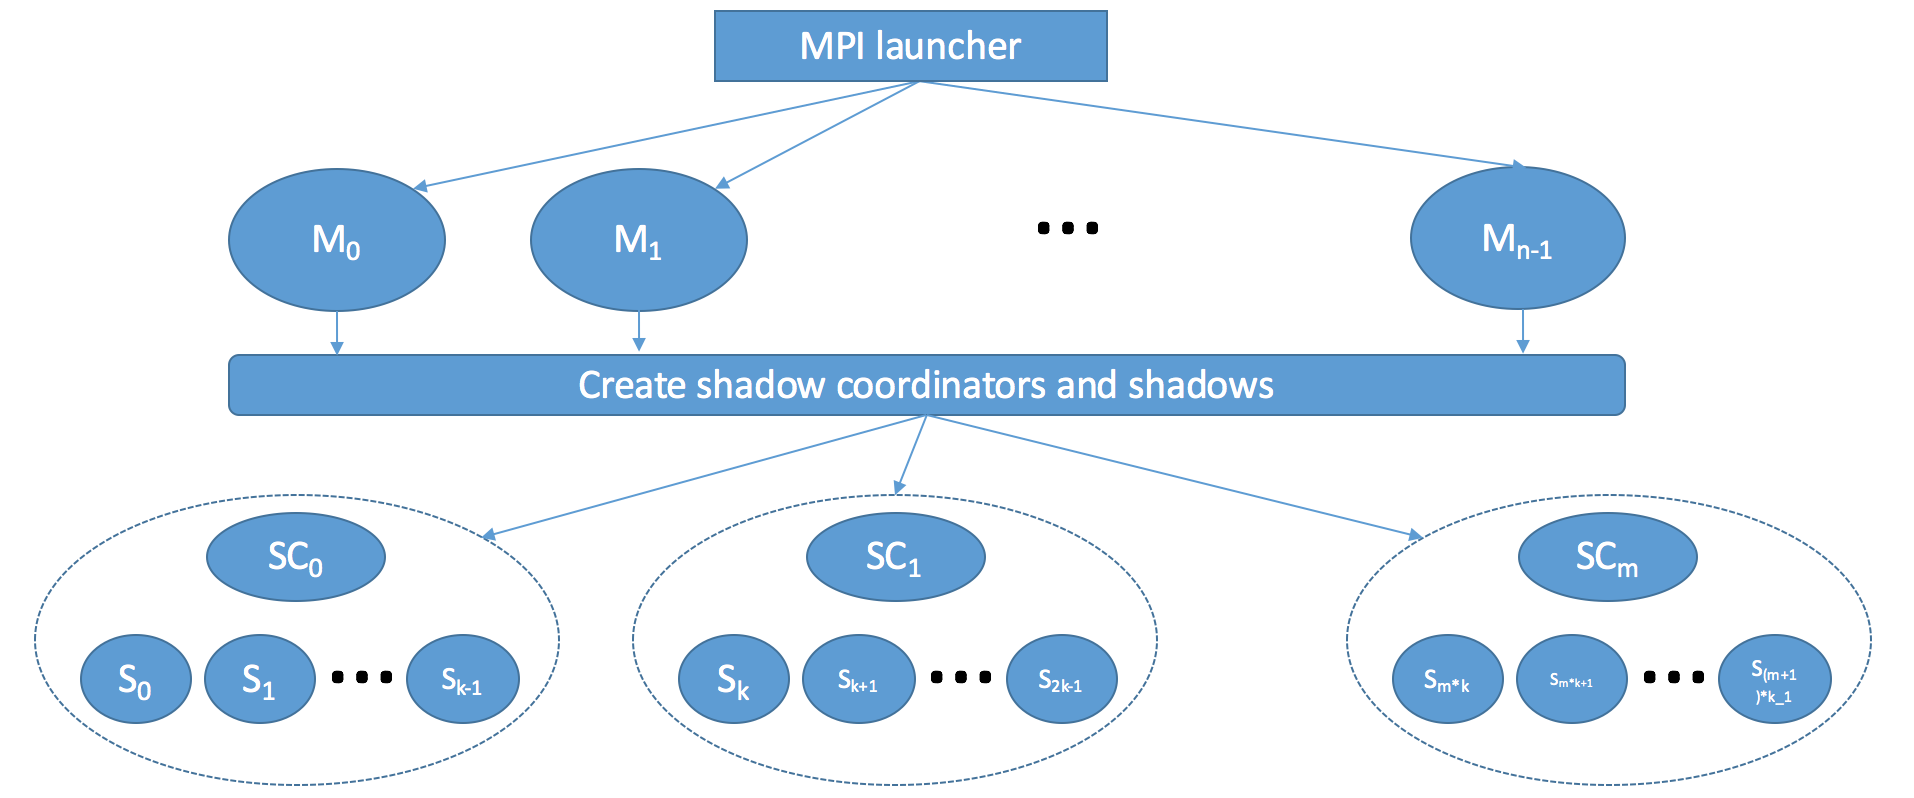
\includegraphics[width=\columnwidth]{figures/logical_org}
  \end{center}
  \caption{Logical organization of a MPI world for Rejuvenating Shadows. $N=16$, $K=4$.}
  \label{fig:logical_org}
\end{figure}

\subsection{Execution rate control}
While the mains always execute at maximum rate for HPC's throughput consideration, the shadows can be configured to execute slower by collocation \cite{cui_2016_scalcom}. 
When using rsMPI, the user has the flexibility to specify the desired collocation ratio (the number of shadows to collocate on each processing unit) through a configuration file that we provide. Accordingly, rsMPI will generate an MPI rankfile and provide it to the MPI runtime to control the process mapping. Note that rsMPI always maps the main and shadow processes of the same task onto different nodes. This is preferred as a fault on a node will not affect both of them. 
%In addition, rsMPI will automatically translate the number of processes (MPI ranks) specified for the application into the number of processes needed by rsMPI. For example, if the user specifies $N$ processes, rsMPI will translate it into $2N + K$ processes, where $K$ is the number of shadowed sets. Therefore, rsMPI will spawn $N$ main processes, $N$ shadow processes, and $K$ shadow coordinator processes for $K$ shadowed sets during MPI initialization. The logical organization is depicted in Figure~\ref{fig:logical_org}. 
To minimize resource usage, each coordinator is collocated with all the shadows in the shadowed set. Since each coordinator simply waits for incoming control messages (discussed below) and does minimal work, it has negligible impact on the execution rate of the collocated shadows. 


\subsection{Coordination between mains and shadows}
Each shadowed set has a coordinator process dedicated to coordination between the main and shadow processes in the shadowed set. 
Coordinators do not execute any application code, but just wait for srMPI defined control messages, and then carry out some 
coordination work accordingly. There are three types of control messages, i.e., termination, failure, and leaping. Correspondingly, each coordinator is responsible for three types of work:
\begin{itemize}
  \item when a main finishes, it notifies its coordinator, which then forces the associated shadow to terminate.
  \item when a main fails, its associated shadow needs to catch up, so the coordinator will temporarily suspend the other collocated shadows, and resume their execution once the recovery is done.
  \item when a main or shadow initiates a leaping, either because of failure or buffer overflow, the coordinator triggers leaping at the associated shadow or main.
\end{itemize}
%Main and shadow processes can communicate with their coordinator via control messages defined by rsMPI. 
% Firstly, when a main process finishes, it notifies its coordinator, which then forces the associated shadow process to terminate. Secondly, when a main process fails, its associated shadow process needs to catch up, so the coordinator will temporarily suspend the other collocated shadows, and resume their execution once the recovery is done. Lastly, when a main or shadow initiates a leaping, either because of failure or buffer overflow, the coordinator triggers leaping at the associated shadow or main.  
%the RAS system will notify the corresponding shadow coordinator, which then promotes the associated shadow process to a new main process and kills the collocated shadows.
To separate control messages from data messages, rsMPI uses a dedicated MPI communicator, created during MPI initialization, for the control messages. In addition, to ensure fast response and minimize the number of messages, coordinators also use OS signals to communicate with their collocated shadows. %There are three types of coordination in srMPI.

\subsection{Message passing and consistency}
We wrapped around every MPI communication function and implemented the consistency protocol described in Section~\ref{sec:shadow}. For sending functions, such as MPI\_Send() and MPI\_Isend(), rsMPI requires the main to duplicate the sending while the shadow does no work. For receiving functions, such as MPI\_Recv() and MPI\_Irecv(), both the main and the shadow does one receiving from the main process at the sending side. Internally, collective communication in rsMPI uses point-to-point communication in a binomial tree topology, which demonstrates excellent scalability.

We assume that only MPI operations can introduce non-determinism, and the SYNC message shown in Figure~\ref{fig:cons_protocol} is introduced to enforce determinism. MPI\_ANY\_SOURCE may result in different message receiving orders between a main and its shadow. To deal with this, we serialize MPI\_ANY\_SOURCE message receiving by having the main first do the receiving and then use a SYNC message to forward the message source information to its shadow, which then issues a receiving with the specific source. Other operations, such as MPI\_Wtime() and MPI\_Probe(), can be dealt with in a similar manner by forwarding the result from a main to its shadow.


\subsection{Leaping}
Checkpointing/restart requires each process to save its execution state, which can be used later to retrieve the computation. Leaping is similar to Checkpointing/restart in saving a process' state, but the state is always transferred between a pair of main and shadow. 
To reduce the size of data involved in saving a process' state, we choose to implement leaping in the same way as application-level checkpointing. rsMPI provides a routine for users to register any data as process state. Application developer could use domain knowledge to identify only necessary state data, or use compiler techniques to automate this~\cite{5160999}. 

rsMPI provides the following API for process state registration:

void leap\_register\_state(void *addr, int count, MPI\_Datatype dt);

For each piece of data to be registered, three parameters are needed: a pointer to the address of the data, the number of data items, and the datatype. Internally, rsMPI uses a linked list to keep track of all registered data. %After each call of ``leap\_register\_state()", rsMPI will add a node to its internal linked list to record the three parameters. 
During leaping, the linked list is traversed to retrieve all registered data as the process state.

Coordination of leaping is easier than coordination of checkpointing, since leaping is always between a pair of main and shadow. To synchronize the leaping between a main and a shadow, the coordinator in the corresponding shadowed set is involved. For example, when a main detects failure of another main and initiates a leaping, it will send a control message to its coordinator, which then uses a signal to notify the associated shadow to participate in the leaping. 

Different from Checkpointing where the process state is saved to storage, leaping directly transfers process state between a main and its shadow. 
Since MPI provides natural support for message passing between processes, 
rsMPI uses MPI messages to transfer process state. Although multiple pieces of data can be registered as a process' state, only a single message is needed to transfer the process state, as MPI supports derived datatypes. To prevent the messages carrying process state from mixing with application messages, rsMPI uses a separate communicator for transferring process state. With the synchronization of leaping by coordinator and the fast transfer of process state via MPI messages, the overhead of leaping is minimized. 

A challenge in leaping lies in the need for maintaining state consistency across leaping. To make sure a pair of main and shadow stay consistent after a leaping, not only user-defined states should be transferred correctly, but also lower level states, such as program counter and message buffer, need to be updated correspondingly. Specifically, the lagging process needs to satisfy two requirements. 
Firstly, after leaping the lagging process should discard all obsolete messages before resuming normal execution. Secondly, the lagging process should resume execution at the same point as the target process. We discuss our solutions below, under the assumption that the application's main body consists of a loop, which is true in most cases. 
%Firstly, after updating its state, the lagging process should resume execution at the same point as the target process. Secondly, the lagging process should discard all obsolete message before resuming normal execution. To address these issues, first we assume that the application's main body consists of a loop, which is true in most cases. 

To satisfy the second requirement, we restrict leaping to always occur at certain possible points, and uses internal counter to make sure that both lagging and target processes start leaping from the same point. For example, when a main process triggers a leaping and asks coordinator to notify its associated shadow, the coordinator will trigger the shadow's specific signal handler. The signal handler does not carry out leaping, but sets a flag for leaping and receives a counter value that indicates the leaping point from its main process. Then, the shadow will check the flag and compare the counter value at every possible leaping point. Only when both the flag is set and counter value matches will the shadow start leaping. In this way, it is guaranteed that after leaping the main and shadow will resume execution from the same point. To balance the trade-off between the implementation overhead and the flexibility of checking for when to perform leaping, we choose MPI receive operations as the possible leaping points. 

There is no straightforward solution for the first problem, as the message buffer is maintained by MPI runtime and not visible to rsMPI. Alternatively, rsMPI borrows the idea of message logging to correctly discard all obsolete messages. During normal execution, both the main and shadow record the meta data (i.e., MPI source, tag, and communicator) for all received messages in the receiving order. During leaping, the meta data at the main is transferred to the shadow, so that the shadow knows about the messages that have been received by its main but not by itself. Then the shadow combines MPI probe and MPI receive operations to remove the messages from MPI runtime buffer in correct order. 

%Alternatively, we choose to remove obsolete message from message buffer by having the process execute all the skipped MPI communication routines after it finishes leaping. To achieve this, we require the user to define a function for the MPI communication functions used in the application's main body loop. The function should have two parameters to specify the starting and ending index for skipped iterations. In addition, the user needs to register the function with rsMPI with the following library call:

%void leap\_register\_func(void (*func)(int, int));

%To discard all obsolete messages after leaping, the process that updates its process state will call the registered function, for which the two parameters will be automatically specified by rsMPI. Essentially, it executes all the  MPI communication functions from the skipped iterations and consumes all the useless messages.  

%\subsection{Failure injection and detection}
%As one main goal of this work is to achieve fault tolerance, an integrated fault injector is required to evaluate the effectiveness and efficiency of rsMPI to tolerate failures during execution. To produce failures in a manner similar to naturally occruing process failures, our failure injector is designed to be distributed and co-exist with all rsMPI processes. Failure is injected by sending a specific signal to the target process.

%Failure detection is beyond the scope of srMPI, and we assume the underlying hardware platform has a RAS system that provides this functionality. In our prototype, we emulate a RAS system with a signal handler installed at every main and shadow process. The signal handler catches failure signal from failure injector, and uses a rsMPI defined failure message via a dedicated communicator to notify all other processes of its failure. Similar to ULFM, processes in srMPI can detect failure only when it does an MPI receive operation. When starting a srMPI receive, srMPI checks for failure messages before it does the actual MPI receive operation.

%\subsection{Double in-memory checkpointing}
%We also implemented checkpointing to compare with srMPI in the presence of failures. To be optimistic, we chose double in-memory checkpointing that is much more scalable then disk-based checkpointing~\cite{zheng2004ftc}. Same as leaping in srMPI, our implementation provides an API for process state registration. This API requires the same parameters as leap\_register\_state(void *addr, int count, MPI\_Datatype dt), but internally, it needs to allocate extra memory in order to store the state of a ``buddy" process. Another provided API is checkpoint(), which can be used to insert a checkpoint in the application code. For fairness, our implementation also uses MPI messages to transfer state between buddies.  